\documentclass[12pt,a4paper]{scrartcl}
\usepackage[english]{babel}
\usepackage{fontspec}
\usepackage{polyglossia}

\usepackage{csquotes}

\usepackage{graphicx}
\usepackage{float}
\usepackage[backend=bibtex,style=numeric]{biblatex}

\usepackage{listings}
\usepackage{xcolor}
\usepackage{enumitem}

\definecolor{darkgreen}{HTML}{006400}


\addbibresource{bibliography.bib}


\setmainfont{DejaVu Sans}
\begin{document}

    \begin{titlepage}
        \titlehead{OTH Regensburg\\
        Computer Science and Mathematics\\}
        \subject{Study Project}
        \subtitle{Course: Compiler Construction}
        \title{Interpreter for the programming language STYX}
        \date{Winter Semester 2022/2023}
        \author{Finn Artmann}
        \maketitle
    \end{titlepage}


    \tableofcontents

    \newpage

    \section{Introduction}
        The programming language "SŦYX" is an esoteric, interpreted programming language,
which mainly uses UTF-8 special characters. It is therefore inherently hard to read.
The syntax is oriented on the programming
language C.  The Interpreter is for SŦYX written in C using "flex"
and "bison" as a lexer and parser generator.
The interpreter builds an abstract syntax tree (AST) while parsing the source code and
executes the AST afterwards. The following chapters will describe the syntax of SŦYX
and the implementation of the interpreter.



    \section{Lexer implementation}
        The lexer is implemented in the file \textit{src/styx.l}. Regarding the
lexer implementation it is important to know how UTF-8 characters are
encoded. Otherwise, there might be hard to debug issues when using
regular expressions to match these characters. Flex scans the input byte-wise,
but UTF-8 characters can be encoded with up to 4 bytes. So when we want to match
a UTF-8 character, we need to make sure we match the whole sequence of bytes.
\newline
Additionally to recognizing keywords, identifiers, operators and other special 
character the lexer is also able to recognize numbers in different formats and
supports linecomments and blockcomments. For those, the lexer tries to take as
much work away from the parser as possible for example by completely
ignoring the content of comments and converting numbers to decimal numbers when
possible. Special number formats will be discussed in more detail in the specific chapter.
\newline
Also supported are String literals, which can still make use of special characters
used elsewhere in the language by escaping them using the defined escape character.
They are also able to span multiple lines with the use of newline symbols.
Strings can also include arbitrary ascii characters by using the escape character.
\newline
Another unconventional feature compared to other programming languages
is that lexemes are not separated by whitespace,
but by the special character \textcolor{teal}{\#} or a newline
to better fit in with the cryptic theme of the language. 

    \section{Syntax}
        To keep this document in the requested length, only a few selected tokens are listed here explicitly.
        To review all tokens recognized by the lexer, please refer to the lexer implementation (\textit{src/styx.l}).
        \subsection{Number formats}
            The lexer can recognize the following number formats:
\begin{itemize}[noitemsep]
    \item Decimal numbers (e.g. \textcolor{teal}{42}) 
    \item Hexadecimal numbers (e.g. \textcolor{teal}{Ex2A})
    \item Real numbers (e.g. \textcolor{teal}{3.14})
    \item Babylonian numbers (e.g. \textcolor{teal}{ EB\{YY \textless{\textless}\}BE })
\end{itemize}
\noindent
Decimal and Real numbers can be used in code in the expected way. Hexadecimal numbers
need to be escaped with the \textcolor{teal}{Ex} prefix.\newline
While the first three are self-explanatory, the Babylonian numbers are a bit more complicated.
They can be used in code like this: 
\begin{center}
    \textcolor{teal}{ EB\{insert\_babylonian\_number\_here\}BE }
\end{center}
\noindent
The Babylonian number is then converted to a decimal number by the lexer.
Valid characters for the babylonian numbers are:
\begin{itemize}[noitemsep]
    \item \textcolor{teal}{Y} equals 1
    \item \textcolor{teal}{\textless} equals 10
    \item Empty space is delimiter for the digits
\end{itemize}
\noindent
The babylonian number system is a positional number system, where the base is 60.
The following table show the representation of the numbers 1 to 59:
%include picture and give add Babylonian as source
\begin{center}
    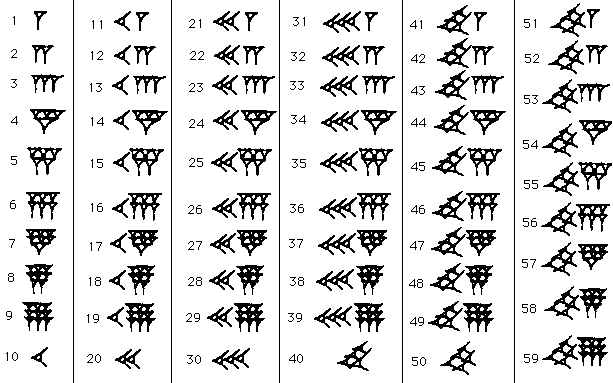
\includegraphics[width=0.5\textwidth]{babylonian_numbers.png}
    \cite{Babylonian}
\end{center}
\noindent








        \subsection{Data types}    
            The supported data types are:
\begin{itemize}[noitemsep]
    \item \textcolor{teal}{ı’Ŧ} (integer)
    \item \textcolor{teal}{ÐØ↑‘Ł€} (double)
    \item \textcolor{teal}{ẞŦ®ı’Ŋ} (string) Usage: \textcolor{teal}{⅜insert\_string\_here⅜}
    \item \textcolor{teal}{©ĦÆ®} (character) Usage: Coming soon, see lexer file
    \item \textcolor{teal}{‚ØıÐ} (void)
\end{itemize}
\noindent
The language has a strong type system, which means that every variable has a type and
the type of a variable can not be changed. The type of a variable is determined on declaration.
Trying to assign a value of a different type to a variable will result in a type mismatch error.


        \subsection{Program structure}
            A SŦYX program is required to have a main function called \textcolor{teal}{ºÆı’}, which is the entry point of the program.
The main function is required to have the return type \textcolor{teal}{ı’Ŧ} and can not have any parameters.
Functions have to be defined above the main function. Any statements
or declarations that are not control structures are terminated by a semicolon.
        \subsection{Functions}
            SŦYX supports functions which can have parameters and a return type.
The return type can be any of the supported data types.
Functions can be called from within the main function or other functions
and can be called recursively. They do not have to be defined in a specific order 
(except before the main function).\newline
At the current state of the language, the return statement does not immediately
stop the execution of the function, but instead returns the value to the caller
at the end of the function. The returned value from a function call can directly
be assigned to a variable of the same type or used as a parameter for another function call.
\newline
Here is some example code which shows the functions "foo" and "bar" and "main".
The function "main" has a print statement with the function call to "foo" as argument,
which itself has the integer 4 as argument. The function "foo" calls the function "bar",
which increments the given integer by 1 and returns it.
\begin{center}
    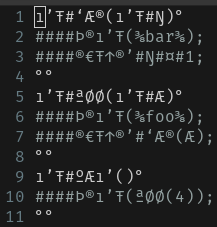
\includegraphics[width=0.3\textwidth]{styx_func.png}
\end{center}

        \subsection{Variables}
            Variables can be of the data types described earlier. 
The variable has to be declared before it can be used.
Declarations can be done anywhere in a function body or in the main function.
A variable can also be declared as global variable using the \textcolor{teal}{ŊŁØ‘ÆŁ} keyword,
which makes it accessible from anywhere in the program.
It is possible to directly assign a value to a variable on declaration.
Local variables can not be accessed from outside the function or the scope they are declared in.
Scopes can be created using \textcolor{teal}{°} and \textcolor{teal}{°°} in any
function body or the main function.
\newline
\newline
Examples Declarations:
\begin{itemize}[noitemsep]
    \item Standard declaration: \textcolor{teal}{ÐØ↑‘Ł€\#‚Æ®;}
    \item Declaration with assignment: \textcolor{teal}{ÐØ↑‘Ł€\#‚Æ®\#§\#3.14;}
\end{itemize}


        \subsection{Control flow}
            Implemented control flow statements are:
\begin{itemize}[noitemsep]
    \item If-Statement : \textcolor{teal}{ıª(}condition\textcolor{teal}{)°}body\textcolor{teal}{°°}
    \item If-Else-Statement: \textcolor{teal}{ıª(}condition\textcolor{teal}{)°}body\textcolor{teal}{°°€Łẞ€°}body\textcolor{teal}{°°}
    \item For-Loop: \textcolor{teal}{ªØ®(}declaration\textcolor{teal}{;}condition\textcolor{teal}{;}increment\textcolor{teal}{)°}body\textcolor{teal}{°°}
\end{itemize}
        \subsection{User I/O and other built-in functions}
            SŦYX has built-in functions for user input and output that work with all supported data types. 
\textcolor{teal}{ẞ©Æ’(}variable\textcolor{teal}{)} reads a value 
from the standard input and assigns it to the variable.
\textcolor{teal}{Þ®ı’Ŧ(}variable\textcolor{teal}{)} prints the value of the variable to the standard output.
There also is the possibility to call the print function with an additional width parameter
like this: \textcolor{teal}{Þ®ı’Ŧ(}width\textcolor{teal}{?}variable\textcolor{teal}{)}
This results in the output being formatted to the specified width.\newline
\newline
Random integers beween 0 and a specified value can be generated using the 
\textcolor{teal}{®Æ’Ðı’Ŧ(}variable\_max\_number\textcolor{teal}{)} function,
which returns the generated number.\newline
\newline
Another built-in function is \textcolor{teal}{ẞ›ẞŦ€º(}variable\_string\textcolor{teal}{)},
which allows the user to call a system command  with a string as parameter.
The return value of this function is 0 if the command was executed successfully and non zero otherwise.
        
    \section{Abstract Syntax Tree}
        The parser builds an abstract syntax tree (AST) while parsing the source code and
        executes the AST afterwards. Available functions can be found in the
        \textit{include/ast.h} header file or in the \textit{src/ast.c} source file.
        \subsection{AST nodes}
            Each node contains the following fields:
\begin{itemize}[noitemsep]
    \item \textbf{id} (int): A unique identifier for the node that is assigned on creation.
    \item \textbf{type} (int): The type of the node specifies the token type of the node.
    \item \textbf{data\_type}: Used to determine the data type of the value stored in the val field.
    \item \textbf{val} (val\_t): Stores the value of the node.
    \item \textbf{is\_const} (int): Used to determine if the node is constant.
    \item \textbf{child} (struct\ astnode\_t*): Stores pointers to the child nodes.
\end{itemize}
        \subsection{Debugging}
            After the AST is executed and fully traversed the parser will generate a
Graphviz file, which can be used to visualize the AST. To display node names 
in a human-readable form, token IDs are converted to their corresponding
token names using the internal token table provided by bison.
There also is a function to print the AST to console.\newline
By setting the pre-compiler directive \textit{\#define DEBUG\_AST} in the header file
each node of the AST will be printed to the console while traversing it.
        \subsection{Optimization}
            Constant folding is implemented for arithmetic operations.
The optimization takes place while the AST is being traversed and is 
implemented in the \textit{operation} function in the \textit{src/ast.c} source file.
When the AST is traversed, and an operation is encountered for the
first time, the operation is evaluated, and the result is stored in the
\textit{value} field of the node. This optimization is only possible if 
all child nodes have a constant value. For this reason each ast node has a
\textit{is\_const} field. A node is marked as constant if all child nodes are
constant. When the original operation node is encountered again, the node is 
marked as constant and \textit{value} field can be used instead of traversing the
child nodes again.



    \newpage
    \printbibliography


\end{document}
